% ============================================================
% MLC Network Detection System -- Optimized Project Report
% MACHINE LEARNING CONCEPT-2 (CSE 3968)
% SIKSHA 'O' ANUSANDHAN (Deemed To Be University)
% ITER, S'O'A | Batch 2023 | Session 2025-26
% ============================================================

\documentclass[11pt,a4paper,oneside]{article}

% ---------- Encoding, Page, Fonts ----------
\usepackage[T1]{fontenc}
\usepackage[utf8]{inputenc}
\usepackage[english]{babel}
\usepackage[top=2cm,bottom=2cm,left=2.4cm,right=1.8cm]{geometry}
\usepackage{lmodern}
\usepackage{microtype}
\usepackage{setspace}
\setstretch{1.12}
\setlength{\parindent}{0pt}
\setlength{\parskip}{3pt}

% ---------- Colors ----------
\usepackage[dvipsnames,table]{xcolor}
\definecolor{SOAblue}{RGB}{0,53,107}
\definecolor{SOAgold}{RGB}{185,141,0}
\definecolor{SOAlightblue}{RGB}{220,234,249}
\definecolor{SOAgray}{RGB}{246,246,246}
\definecolor{SOAsoft}{RGB}{252,252,248}
\definecolor{codegreen}{RGB}{34,120,34}
\definecolor{codegray}{RGB}{120,120,120}
\definecolor{codeblue}{RGB}{0,0,180}
\definecolor{codered}{RGB}{160,0,0}
\definecolor{codebg}{RGB}{248,248,250}

% ---------- Section Formatting ----------
\usepackage{titlesec}
\titleformat{\section}{\large\bfseries\color{SOAblue}}{\thesection.}{0.6em}{}[\vspace{-2pt}\rule{\linewidth}{0.5pt}]
\titleformat{\subsection}{\normalsize\bfseries\color{SOAgold}}{\thesubsection}{0.6em}{}
\titleformat{\subsubsection}{\normalsize\bfseries\itshape\color{SOAblue}}{\thesubsubsection}{0.5em}{}
\titlespacing{\section}{0pt}{8pt}{4pt}
\titlespacing{\subsection}{0pt}{6pt}{2pt}
\titlespacing{\subsubsection}{0pt}{4pt}{1pt}

% ---------- Header / Footer ----------
\usepackage{fancyhdr}
\pagestyle{fancy}
\fancyhf{}
\fancyhead[L]{\small\textcolor{SOAblue}{\textbf{MLC Network Detection System}}}
\fancyhead[R]{\small\textcolor{SOAgold}{\textbf{CSE 3968 | ITER, S'O'A}}}
\fancyfoot[C]{\small\thepage}
\renewcommand{\headrulewidth}{0.5pt}
\renewcommand{\footrulewidth}{0.3pt}

% ---------- Tables ----------
\usepackage{booktabs}
\usepackage{longtable}
\usepackage{tabularx}
\usepackage{array}
\usepackage{colortbl}
\usepackage{makecell}
\usepackage{ragged2e}
\newcolumntype{Y}{>{\RaggedRight\arraybackslash}X}
\newcolumntype{L}[1]{>{\RaggedRight\arraybackslash}p{#1}}
\newcolumntype{C}[1]{>{\Centering\arraybackslash}p{#1}}
\newcolumntype{R}[1]{>{\RaggedLeft\arraybackslash}p{#1}}
\renewcommand{\arraystretch}{1.22}
\setlength{\tabcolsep}{4pt}

% ---------- Code Listings ----------
\usepackage{listings}
\lstdefinestyle{pycode}{
  language=Python,
  backgroundcolor=\color{codebg},
  basicstyle=\ttfamily\scriptsize,
  keywordstyle=\bfseries\color{codeblue},
  commentstyle=\itshape\color{codegreen},
  stringstyle=\color{codered},
  numberstyle=\tiny\color{codegray},
  numbers=left,
  numbersep=6pt,
  tabsize=4,
  breaklines=true,
  breakatwhitespace=false,
  showstringspaces=false,
  frame=single,
  framerule=0.4pt,
  rulecolor=\color{SOAblue!30},
  xleftmargin=14pt,
  xrightmargin=2pt,
  captionpos=b,
  aboveskip=4pt,
  belowskip=4pt
}
\lstdefinestyle{bashcode}{
  language=bash,
  backgroundcolor=\color{black!86},
  basicstyle=\ttfamily\scriptsize\color{white},
  keywordstyle=\bfseries\color{yellow},
  breaklines=true,
  frame=none,
  xleftmargin=10pt,
  numbers=none,
  aboveskip=4pt,
  belowskip=4pt
}
\lstset{style=pycode}
\renewcommand{\lstlistingname}{Code}

% ---------- Graphics and Frames ----------
\usepackage{graphicx}
\usepackage{float}
\usepackage{caption}
\usepackage{subcaption}
\captionsetup{font=small,labelfont={bf,color=SOAblue},skip=4pt}
\graphicspath{{./}{report_assets/}}

\usepackage{mdframed}
\mdfdefinestyle{imgbox}{
  linecolor=SOAblue!40,
  linewidth=0.8pt,
  backgroundcolor=SOAlightblue!18,
  innertopmargin=6pt,
  innerbottommargin=6pt,
  innerleftmargin=6pt,
  innerrightmargin=6pt,
  roundcorner=3pt
}
\mdfdefinestyle{infobox}{
  linecolor=SOAgold,
  linewidth=1pt,
  backgroundcolor=SOAgold!7,
  innertopmargin=6pt,
  innerbottommargin=6pt,
  innerleftmargin=8pt,
  innerrightmargin=8pt,
  roundcorner=4pt
}

% ---------- Misc ----------
\usepackage{enumitem}
\setlist{noitemsep,topsep=3pt,parsep=1pt}
\usepackage{amsmath,amssymb}
\usepackage{hyperref}
\hypersetup{
  colorlinks=true,
  linkcolor=SOAblue,
  urlcolor=SOAgold,
  citecolor=SOAblue,
  pdftitle={MLC Network Detection System},
  pdfauthor={ITER, S'O'A}
}
\usepackage{tocloft}
\renewcommand{\cftsecfont}{\bfseries\color{SOAblue}}
\renewcommand{\cftsecpagefont}{\bfseries\color{SOAblue}}

\begin{document}

% ============================================================
% COVER PAGE
% ============================================================
\thispagestyle{empty}
\begin{center}

\colorbox{SOAblue}{\parbox{\linewidth}{\centering\vspace{6pt}
  \textcolor{white}{\Large\bfseries SIKSHA `O' ANUSANDHAN}\\[3pt]
  \textcolor{SOAgold}{\small (Deemed To Be University)}\\[1pt]
  \textcolor{white}{\small Accredited (3rd Cycle) by NAAC with \textbf{A++ Grade}}\\[1pt]
  \textcolor{white}{\small Admission Batch: 2023 \quad|\quad Session: 2025--26}
  \vspace{6pt}
}}

\vspace{0.55cm}
{\large\bfseries\color{SOAblue} Major Project Report of}\\[4pt]
\colorbox{SOAgold!20}{\parbox{0.82\linewidth}{\centering
  \textbf{\large MACHINE LEARNING CONCEPT-2 (CSE 3968)}
}}

\vspace{0.4cm}{\normalsize\bfseries On}\vspace{0.25cm}

\begin{mdframed}[style=infobox]
\centering
{\LARGE\bfseries\color{SOAblue} MLC Network Detection System}\\[5pt]
{\large\color{SOAgold} Network Anomaly Detection Using Machine Learning}\\[3pt]
{\small\color{gray}IoT-23 Dataset | Bagging | Boosting | Random Forest | Isolation Forest | One-Class SVM | Autoencoder | Streamlit}
\end{mdframed}

\vspace{0.4cm}{\normalsize\bfseries Submitted by:}\vspace{0.2cm}

\begin{tabular}{|L{5.7cm}|C{4.2cm}|}
  \hline
  \rowcolor{SOAlightblue}
  \textbf{Name} & \textbf{Registration Number}\\\hline
  NAME 1 & 2341\_\_\_\_\_ \\\hline
  NAME 2 & 2341\_\_\_\_\_ \\\hline
  NAME 3 & 2341\_\_\_\_\_ \\\hline
  NAME 4 & 2341\_\_\_\_\_ \\\hline
\end{tabular}

\vspace{0.4cm}
{\small\textbf{Section:} 2341\_\_\_ \quad \textbf{Semester:} \_\_\_\_\_\_\_ \quad
\textbf{Branch:} Computer Science \& Engineering}

\vspace{0.5cm}
\colorbox{SOAblue!15}{\parbox{3cm}{\centering\vspace{0.55cm}
  \textcolor{SOAblue}{\small\bfseries SOA LOGO}\vspace{0.55cm}}}

\vspace{0.25cm}
{\small\bfseries Department of Computer Science \& Engineering}\\
{\small Institute of Technical Education and Research (ITER), S'O'A}\\
{\small Jagamohan Nagar, Jagamara, Bhubaneswar, Odisha -- 751030}

\vspace{0.35cm}
\colorbox{SOAgold}{\textcolor{white}{\textbf{\normalsize May, 2026}}}
\end{center}

% ============================================================
% CERTIFICATE
% ============================================================
\newpage
\begin{center}{\LARGE\bfseries\color{SOAblue} CERTIFICATE}\end{center}

This is to certify that the Major Project Report titled \textbf{``MLC Network Detection System: Network Anomaly Detection Using Machine Learning''} submitted by the students listed below has been carried out under the supervision of the undersigned and is a bonafide record of work done in partial fulfilment of the requirements of \textbf{Machine Learning Concept-2 (CSE 3968)}, academic session 2025--26.

\vspace{6pt}
\begin{center}
\begin{tabular}{|L{5.2cm}|C{4.6cm}|}
  \hline
  \rowcolor{SOAlightblue}\textbf{Name} & \textbf{Registration No.}\\\hline
  NAME 1 & 2341\_\_\_\_\_\\\hline
  NAME 2 & 2341\_\_\_\_\_\\\hline
  NAME 3 & 2341\_\_\_\_\_\\\hline
  NAME 4 & 2341\_\_\_\_\_\\\hline
\end{tabular}
\end{center}

\vspace{2cm}
\begin{minipage}{0.48\textwidth}
  \textbf{Supervisor / Faculty Guide}\\[0.2cm]
  Name: \underline{\hspace{4cm}}\\[0.15cm]
  Designation: \underline{\hspace{3.5cm}}\\[0.15cm]
  Dept: CSE, ITER, S'O'A
\end{minipage}\hfill
\begin{minipage}{0.45\textwidth}
  \textbf{Head of Department}\\[0.2cm]
  Name: \underline{\hspace{4cm}}\\[0.15cm]
  Designation: Professor \& HOD\\[0.15cm]
  Dept: CSE, ITER, S'O'A
\end{minipage}

\vspace{0.8cm}
\textbf{Date:} \underline{\hspace{3cm}} \hfill \textbf{Place:} Bhubaneswar, Odisha

% ============================================================
% ABSTRACT
% ============================================================
\newpage
\begin{center}{\large\bfseries\color{SOAblue} ABSTRACT}\end{center}

The \textbf{MLC Network Detection System} is a machine learning-based network anomaly detection framework designed to classify network traffic as \textit{Benign} or \textit{Malicious}. Traditional signature-based Intrusion Detection Systems are effective for known attacks but fail when attack behavior changes or when zero-day threats appear. This project uses machine learning to learn traffic behavior from the \textbf{IoT-23 dataset}, a real-world collection of benign and malicious IoT network connection logs.

The pipeline includes dataset loading, data cleaning, Exploratory Data Analysis, feature engineering, preprocessing, model training, evaluation, model saving using \texttt{.pkl}, and Streamlit web deployment. A sample of \textbf{50,000 connection records} was used. Multiple models were trained and compared, including Bagging, Boosting, Isolation Forest, One-Class SVM, Autoencoder, and Random Forest.

\textbf{Key Results:} Random Forest achieved Accuracy 0.9979, Precision 0.9962, Recall 1.0000, and F1-Score 0.9981. The saved model was integrated into a Streamlit app that supports manual traffic prediction and row-wise prediction from \texttt{testing\_data.csv}.

\textbf{Keywords:} Network Anomaly Detection, IoT-23, Random Forest, Isolation Forest, One-Class SVM, Autoencoder, Ensemble Learning, Streamlit, Intrusion Detection, Feature Engineering.

\newpage
\tableofcontents
\newpage
\listoffigures
\listoftables

% ============================================================
\newpage
\section{Introduction}

\subsection{Background}
Cybersecurity is one of the most important areas in modern computing. As IoT devices, cloud platforms, smart infrastructure, and enterprise networks grow, the number of cyberattacks also increases. Attackers use port scanning, malware communication, botnets, denial-of-service attacks, unauthorized access attempts, and command-and-control communication to compromise systems.

Traditional Intrusion Detection Systems depend heavily on predefined signatures. These systems detect known attacks, but they are weak against unknown or zero-day attacks. Machine learning can improve this by learning patterns from historical network traffic and detecting unusual behavior.

\subsection{Project Overview}
The \textbf{MLC Network Detection System} is an end-to-end project that trains machine learning models on IoT network traffic and deploys the best model through a Streamlit web application. The model predicts whether a connection is \textbf{Benign} or \textbf{Malicious}.

\subsection{Why IoT-23 Dataset?}
The IoT-23 dataset contains real IoT malware and benign traffic scenarios. It is more suitable for modern IoT security research than older benchmark datasets because it includes realistic Zeek/Bro network logs and real malware family behavior.

% ============================================================
\section{Problem Statement}

Modern networks generate large volumes of connection logs. Manually analyzing every network record is impossible. Traditional IDS tools face the following issues:

\begin{itemize}
  \item They depend on known signatures.
  \item They cannot reliably detect zero-day attacks.
  \item They require frequent manual rule updates.
  \item They may generate false positives.
  \item They struggle with large-scale IoT traffic.
  \item Malware behavior changes over time.
\end{itemize}

\textbf{Core Problem:} Build a machine learning system that learns from IoT network traffic and classifies a connection as \textbf{Benign} or \textbf{Malicious}, then deploy the saved model through an interactive Streamlit web application.

% ============================================================
\section{Objectives}

The objectives of this project are correct and aligned with the implemented system:

\begin{enumerate}
  \item Load and understand the IoT-23 network traffic dataset.
  \item Use a 50,000-row sample for efficient experimentation.
  \item Clean missing, invalid, and mixed-type values in Zeek logs.
  \item Perform EDA to understand traffic patterns, class distribution, feature distribution, and correlation.
  \item Engineer network-behavior features such as total bytes, total packets, byte ratios, packet ratios, missing-value indicators, and port behavior.
  \item Train and compare Bagging, Boosting, Random Forest, Isolation Forest, One-Class SVM, and Autoencoder models.
  \item Evaluate models using Accuracy, Precision, Recall, F1-score, and Confusion Matrix.
  \item Save the best-performing model as a reusable \texttt{.pkl} file.
  \item Build a Streamlit application for manual prediction and test-data row prediction.
  \item Visualize model output and traffic properties in the application.
\end{enumerate}

% ============================================================
\section{Dataset Description and Understanding}

\subsection{Dataset Used}
The project uses the \textbf{IoT-23 Dataset}, which contains real benign and malicious IoT traffic. The notebook uses the Zeek/Bro connection log file:

\begin{lstlisting}[style=bashcode]
opt/Malware-Project/BigDataset/IoTScenarios/
CTU-IoT-Malware-Capture-1-1/bro/conn.log.labeled
\end{lstlisting}

Only 50,000 rows were loaded to make training practical:

\begin{lstlisting}[style=pycode]
SAMPLE_SIZE = 50_000
\end{lstlisting}

\subsection{Dataset Columns}

\small
\begin{longtable}{|L{3.2cm}|L{10.6cm}|}
\caption{IoT-23 Zeek Connection Log Column Description}
\label{tab:dataset_cols}\\
\hline
\rowcolor{SOAlightblue}
\textbf{Column} & \textbf{Meaning}\\
\hline
\endfirsthead
\hline
\rowcolor{SOAlightblue}
\textbf{Column} & \textbf{Meaning}\\
\hline
\endhead
\texttt{ts} & Unix timestamp of the network connection.\\\hline
\texttt{uid} & Unique connection ID. It is useful for logging but removed during model training.\\\hline
\texttt{id.orig\_h} & Origin/source IP address.\\\hline
\texttt{id.orig\_p} & Origin/source port number.\\\hline
\texttt{id.resp\_h} & Response/destination IP address.\\\hline
\texttt{id.resp\_p} & Response/destination port number.\\\hline
\texttt{proto} & Transport protocol such as TCP, UDP, or ICMP.\\\hline
\texttt{service} & Application service such as HTTP, DNS, SSH, or missing service.\\\hline
\texttt{duration} & Duration of the connection.\\\hline
\texttt{orig\_bytes} & Bytes sent by origin host.\\\hline
\texttt{resp\_bytes} & Bytes sent by response host.\\\hline
\texttt{conn\_state} & Zeek connection state, such as S0, SF, REJ, RSTO.\\\hline
\texttt{missed\_bytes} & Bytes missed during capture.\\\hline
\texttt{history} & Packet history pattern.\\\hline
\texttt{orig\_pkts} & Packets sent by origin host.\\\hline
\texttt{resp\_pkts} & Packets sent by response host.\\\hline
\texttt{label} & Raw traffic label containing benign or malicious information.\\\hline
\end{longtable}
\normalsize

\subsection{Target Variable}
The raw \texttt{label} column was converted into a clean binary target:

\begin{center}
\colorbox{SOAlightblue}{\parbox{0.75\linewidth}{\centering
\textbf{Benign} = normal traffic \qquad \textbf{Malicious} = attack/anomaly traffic}}
\end{center}

% ============================================================
\section{Data Preprocessing}

\subsection{Preprocessing Need}
The dataset contains missing values represented by symbols such as \texttt{-}, empty strings, and \texttt{(empty)}. Some numeric columns are read as object type because of mixed values. Preprocessing is necessary so the models receive clean, numeric, and consistent input.

\subsection{Preprocessing Steps}

\small
\begin{longtable}{|L{3.2cm}|L{3.5cm}|L{7.2cm}|}
\caption{Preprocessing Steps and Justification}
\label{tab:preprocess}\\
\hline
\rowcolor{SOAlightblue}
\textbf{Step} & \textbf{Applied To} & \textbf{Reason}\\
\hline
\endfirsthead
\hline
\rowcolor{SOAlightblue}
\textbf{Step} & \textbf{Applied To} & \textbf{Reason}\\
\hline
\endhead
Missing value conversion & Raw Zeek fields & Converts \texttt{-}, blank values, and \texttt{(empty)} into proper missing values.\\\hline
Numeric coercion & Byte, packet, duration, and port fields & Ensures mathematical operations and model training can be performed correctly.\\\hline
Median imputation & Numeric columns & Handles missing numeric values while reducing outlier effect.\\\hline
Most frequent imputation & Categorical columns & Fills missing category values using the most common class.\\\hline
One-hot encoding & Categorical columns & Converts protocol, service, state, history, and prefix values into model-readable numeric columns.\\\hline
Standard scaling & Numeric columns & Improves model stability, especially for SVM and Autoencoder.\\\hline
Train-test split & Full dataset & Splits 80\% for training and 20\% for testing using stratification.\\\hline
\end{longtable}
\normalsize

% ============================================================
\section{Exploratory Data Analysis}

\subsection{EDA Purpose}
EDA was performed to understand class distribution, missing values, numeric feature behavior, and relationships between features. This is important because network attack patterns are often visible through abnormal byte count, packet count, connection duration, missing response, or unusual port behavior.

\subsection{Class Distribution}

\begin{figure}[H]
\centering
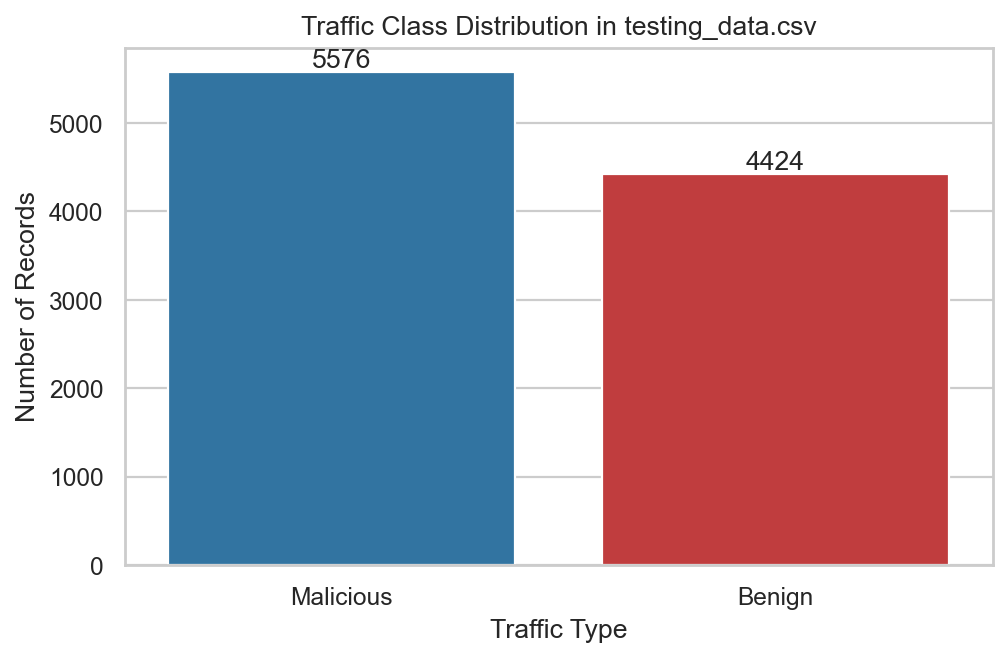
\includegraphics[width=12.5cm,height=7.2cm,keepaspectratio]{fig_01_class_distributio.jpeg}
\caption{Benign vs Malicious traffic distribution in testing data.}
\label{fig:classdist}
\end{figure}

The class distribution helps us understand whether the model could be biased toward one class. In network security, even if the dataset is moderately imbalanced, recall remains important because missing malicious traffic is risky.

\subsection{Numeric Feature Distributions}

\begin{figure}[H]
\centering
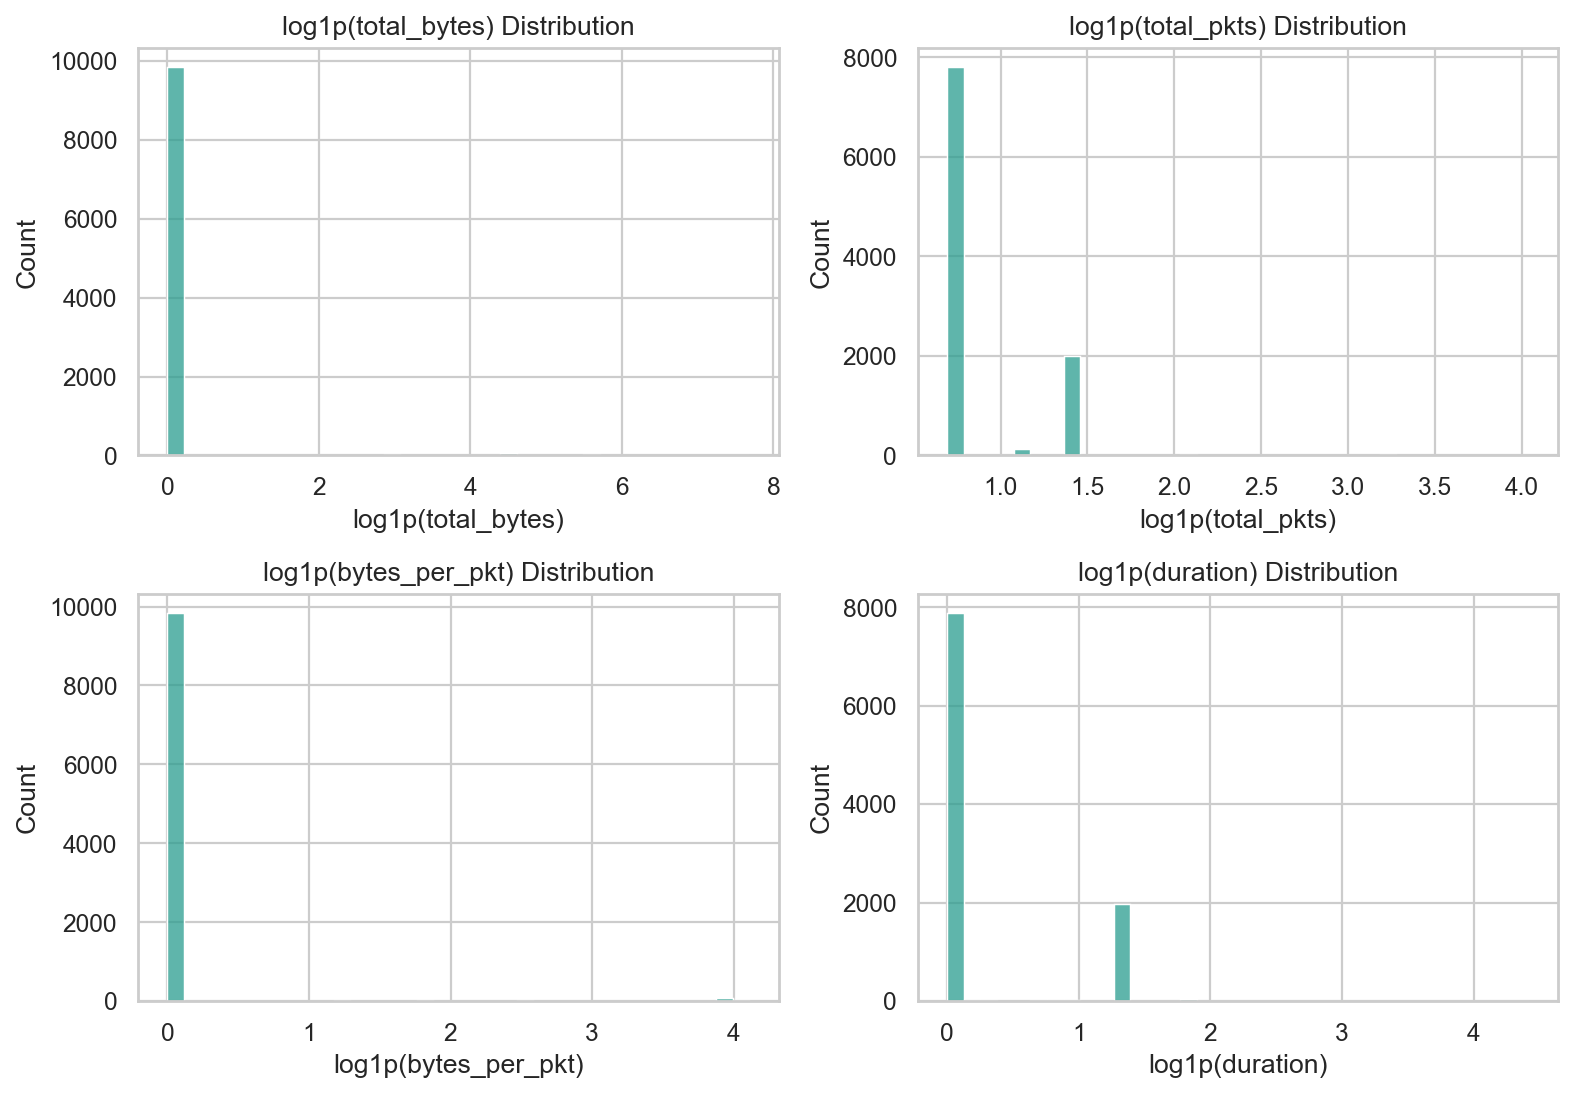
\includegraphics[width=15.0cm,height=9.0cm,keepaspectratio]{fig_02_numeric_distributions.png}
\caption{Distribution of key numeric traffic features using log transformation.}
\label{fig:numdist}
\end{figure}

Network traffic values are usually skewed. For example, most connections may transfer very few bytes, while a few connections transfer large amounts. Log transformation helps reveal the hidden distribution pattern.

\subsection{Correlation Heatmap}

\begin{figure}[H]
\centering
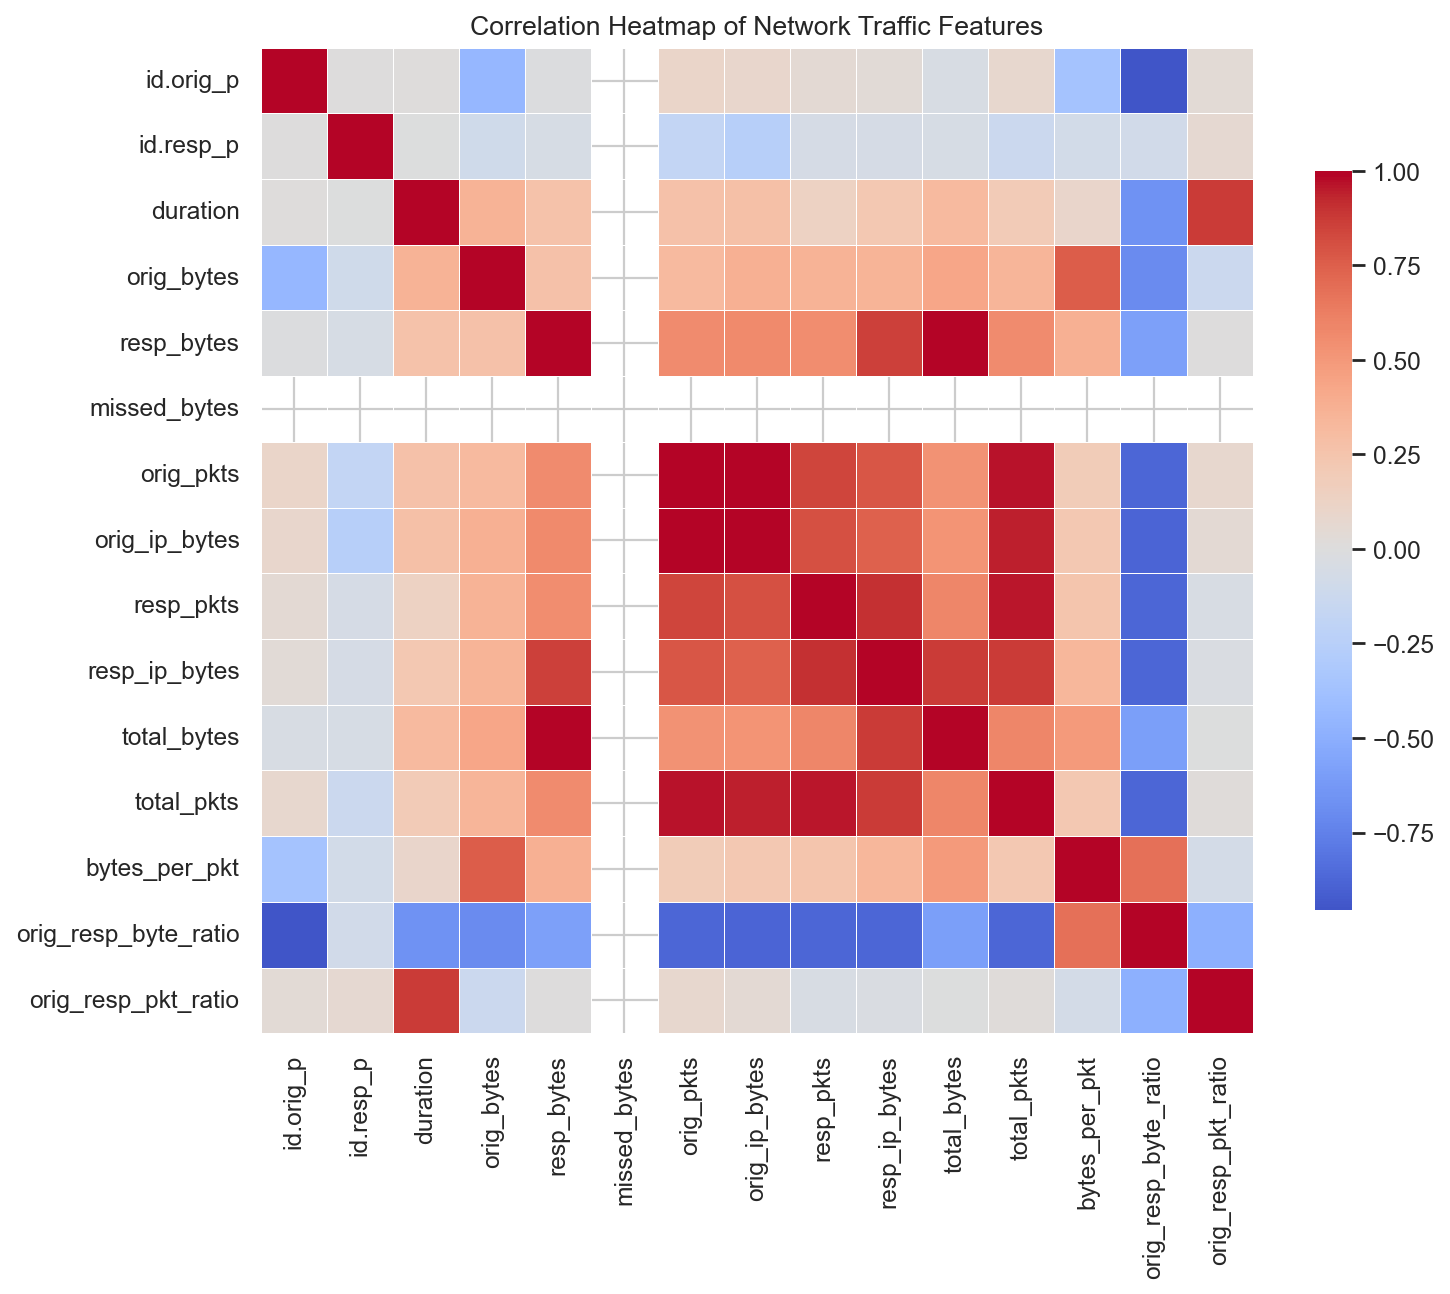
\includegraphics[width=14.0cm,height=10.0cm,keepaspectratio]{fig_03_correlation_heatmap.png}
\caption{Correlation heatmap of network traffic features.}
\label{fig:corr}
\end{figure}

The heatmap shows that packet-related and byte-related features are related. This supports the idea that engineered features such as total packets, total bytes, and byte-per-packet ratio can improve model performance.

\subsection{EDA Intuition}
\begin{mdframed}[style=infobox]
\textbf{EDA Intuition:}
\begin{itemize}
  \item Malicious scanning traffic often has low duration, low bytes, and repeated failed connection states.
  \item Malware communication may target specific destination ports repeatedly.
  \item Missing service or response bytes can indicate incomplete, rejected, or suspicious connections.
  \item Packet and byte ratios help detect asymmetric communication such as one-way scanning or command-and-control behavior.
\end{itemize}
\end{mdframed}

% ============================================================
\section{Feature Engineering}

\subsection{Why Feature Engineering Was Required}
Raw network fields do not always directly show attack behavior. Feature engineering converts raw columns into behavioral signals. For example, \texttt{orig\_bytes} and \texttt{resp\_bytes} separately give volume information, but \texttt{orig\_resp\_byte\_ratio} explains communication imbalance.

\small
\begin{longtable}{|L{4.1cm}|L{4.2cm}|L{5.5cm}|}
\caption{Engineered Features and Their Security Importance}
\label{tab:features}\\
\hline
\rowcolor{SOAlightblue}
\textbf{Feature} & \textbf{Meaning} & \textbf{Why It Helps}\\
\hline
\endfirsthead
\hline
\rowcolor{SOAlightblue}
\textbf{Feature} & \textbf{Meaning} & \textbf{Why It Helps}\\
\hline
\endhead
\texttt{service\_missing} & Whether service is missing & Missing service often occurs in failed scans or incomplete connections.\\\hline
\texttt{history\_missing} & Whether packet history is missing & Incomplete history may indicate abnormal capture or traffic behavior.\\\hline
\texttt{orig\_bytes\_missing} & Missing origin bytes flag & May indicate failed or one-sided traffic.\\\hline
\texttt{resp\_bytes\_missing} & Missing response bytes flag & No response can occur during scanning or blocked malicious attempts.\\\hline
\texttt{hour} & Hour extracted from timestamp & Captures time-based attack behavior.\\\hline
\texttt{dayofweek} & Day of week from timestamp & Captures periodic traffic behavior.\\\hline
\texttt{total\_bytes} & Origin + response bytes & Measures total connection data volume.\\\hline
\texttt{total\_pkts} & Origin + response packets & Measures total packet activity.\\\hline
\texttt{bytes\_per\_pkt} & Average packet size & Detects abnormal packet-size patterns.\\\hline
\texttt{orig\_resp\_byte\_ratio} & Origin/response byte ratio & Detects asymmetric communication and possible scanning.\\\hline
\texttt{orig\_resp\_pkt\_ratio} & Origin/response packet ratio & Detects packet-level imbalance.\\\hline
\texttt{resp\_port\_is\_well\_known} & Destination port $\leq$ 1024 & Identifies common attack targets such as SSH, Telnet, HTTP.\\\hline
\texttt{orig\_ip\_prefix} & Source network prefix & Captures subnet-level behavior without using full IP.\\\hline
\texttt{resp\_ip\_prefix} & Destination network prefix & Captures target network pattern.\\\hline
\end{longtable}
\normalsize

\subsection{Feature Importance}

\begin{figure}[H]
\centering
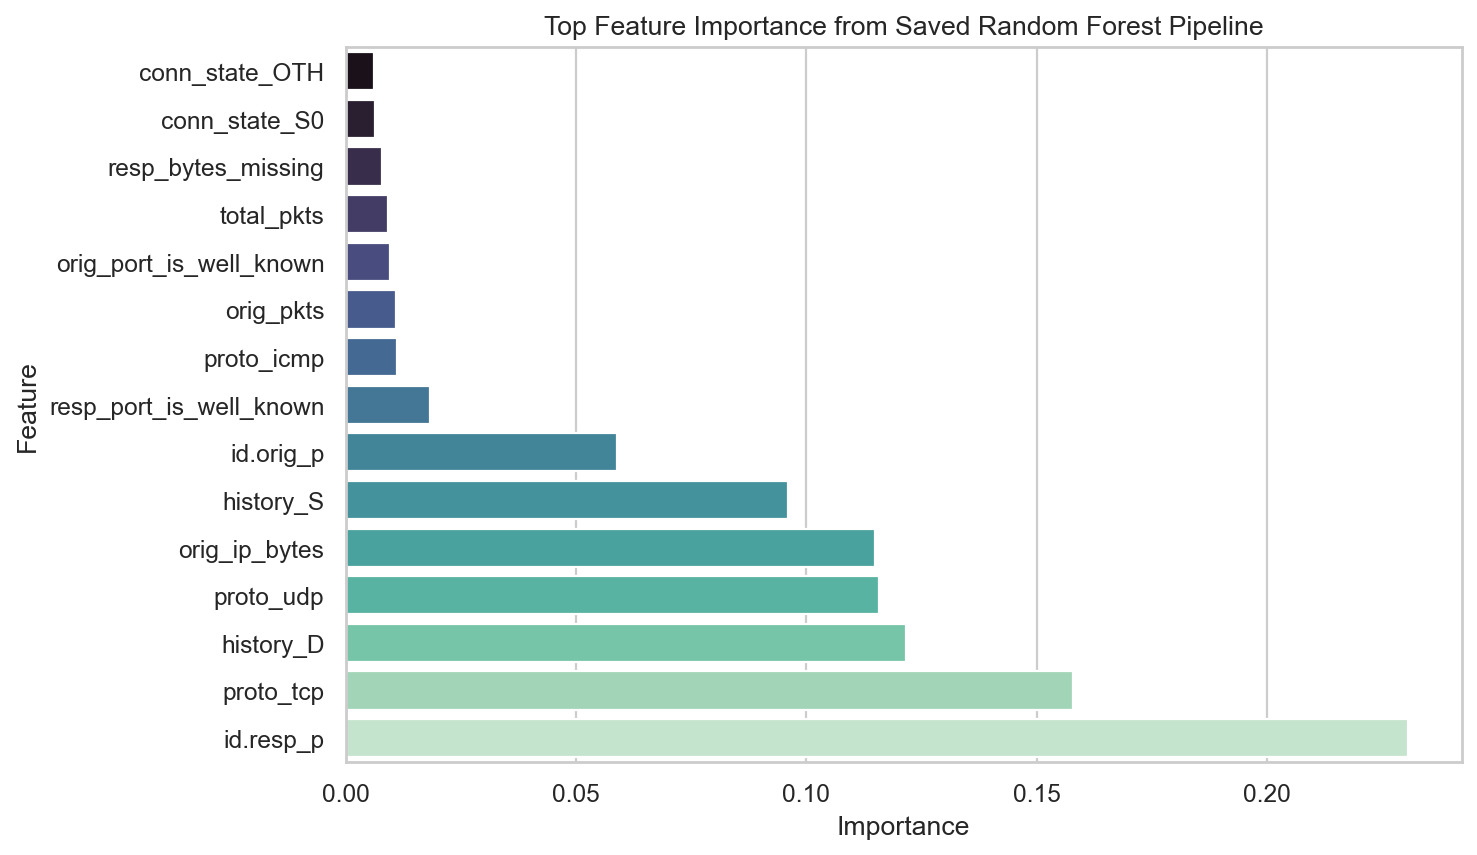
\includegraphics[width=14.0cm,height=8.2cm,keepaspectratio]{fig_06_feature_importance.png}
\caption{Top feature importance values from the saved Random Forest model.}
\label{fig:featimp}
\end{figure}

The feature importance graph shows that the Random Forest model relies strongly on network behavior indicators such as port-related features, connection state, packet count, and byte count. This aligns with the EDA intuition that attacks often differ from normal traffic through communication imbalance, port behavior, and missing or failed responses.

% ============================================================
\section{Implementation}

\subsection{Implementation Steps}

\begin{enumerate}
  \item \textbf{Dataset Loading:} Loaded the IoT-23 connection log using Pandas with explicit column names and missing-value indicators.
  \item \textbf{Target Cleaning:} Converted raw labels into \texttt{Benign} and \texttt{Malicious}.
  \item \textbf{EDA:} Generated class distribution, numeric distribution, and correlation heatmap.
  \item \textbf{Feature Engineering:} Created missing flags, time features, byte/packet aggregates, traffic ratios, port flags, and IP prefixes.
  \item \textbf{Train-Test Split:} Used 80/20 stratified split to preserve label distribution.
  \item \textbf{Preprocessing Pipeline:} Used \texttt{ColumnTransformer} for numeric and categorical preprocessing.
  \item \textbf{Model Training:} Trained Bagging, Boosting, Random Forest, Isolation Forest, One-Class SVM, and Autoencoder models.
  \item \textbf{Evaluation:} Compared models using accuracy, precision, recall, F1-score, and confusion matrix.
  \item \textbf{Model Saving:} Saved the best Random Forest pipeline as \texttt{best\_network\_anomaly\_model.pkl}.
  \item \textbf{Streamlit Deployment:} Built \texttt{app.py} to load the saved model and provide manual and CSV-row prediction.
\end{enumerate}

\subsection{Technology Stack}

\small
\begin{longtable}{|L{4.2cm}|L{9.5cm}|}
\caption{Technology Stack Used}
\label{tab:tech}\\
\hline
\rowcolor{SOAlightblue}
\textbf{Category} & \textbf{Technology}\\
\hline
\endfirsthead
\hline
\rowcolor{SOAlightblue}
\textbf{Category} & \textbf{Technology}\\
\hline
\endhead
Programming Language & Python\\\hline
Notebook Environment & Jupyter Notebook / Google Colab\\\hline
Data Processing & Pandas, NumPy\\\hline
Visualization & Matplotlib, Seaborn, Plotly\\\hline
Machine Learning & Scikit-learn\\\hline
Deep Learning & TensorFlow / Keras\\\hline
Model Persistence & Joblib, Pickle\\\hline
Web Application & Streamlit\\\hline
Dataset & IoT-23 Dataset\\\hline
\end{longtable}
\normalsize

\subsection{System Architecture}

\begin{figure}[H]
\centering
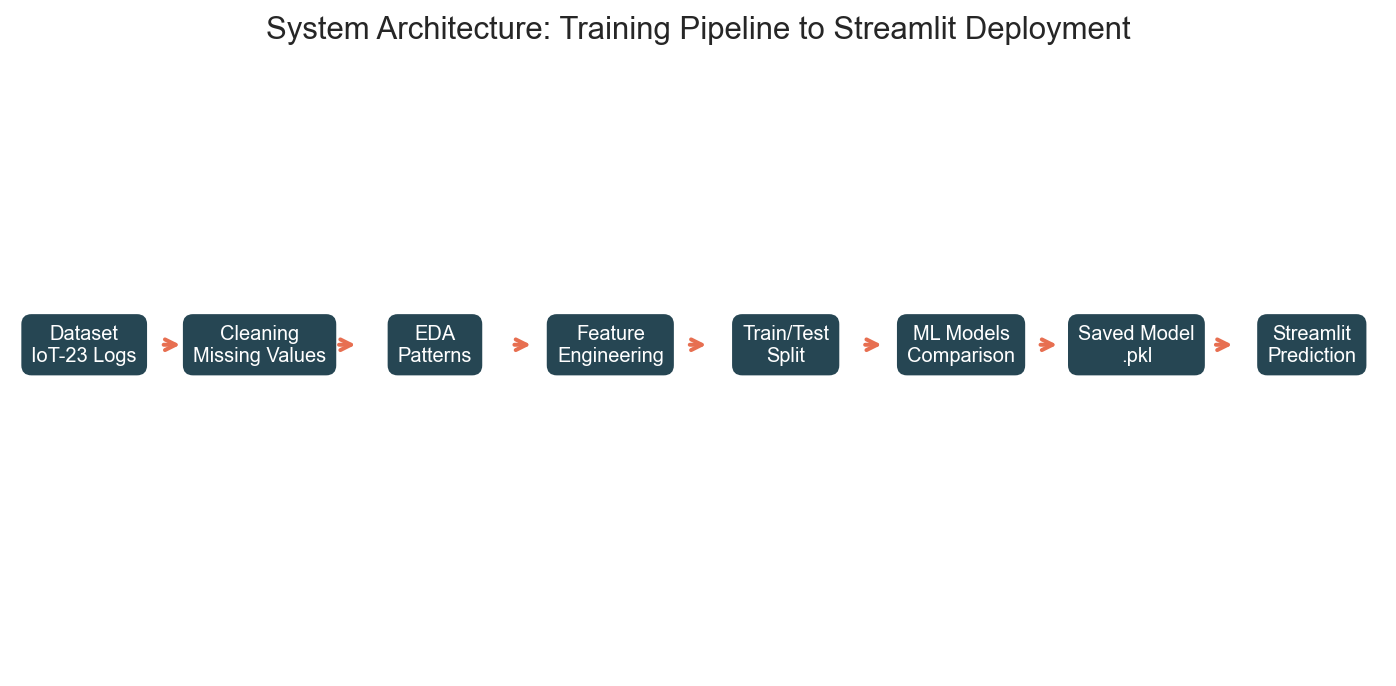
\includegraphics[width=0.95\linewidth]{fig_07_system_architecture.png}
\caption{System architecture from dataset loading to Streamlit deployment.}
\label{fig:architecture}
\end{figure}

\subsection{Streamlit Workflow}

\begin{figure}[H]
\centering
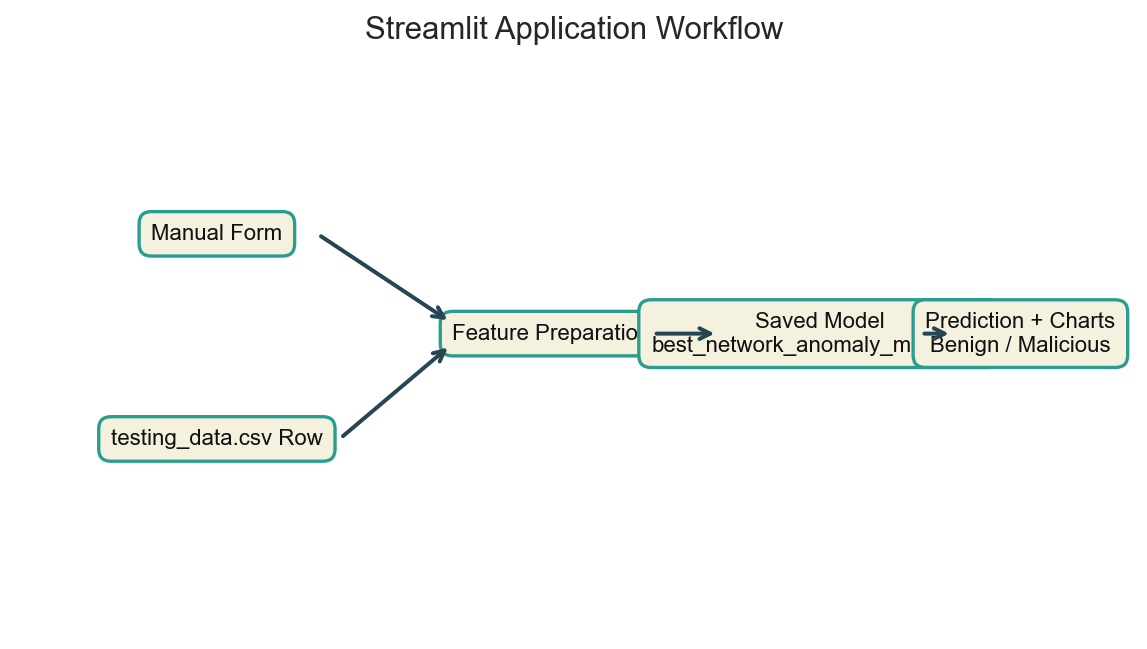
\includegraphics[width=0.9\linewidth]{fig_08_streamlit_workflow.png}
\caption{Streamlit workflow for manual input and testing-data row prediction.}
\label{fig:streamlitflow}
\end{figure}

% ============================================================
\section{Model Development and Justification}

\subsection{Models Used}

\small
\begin{longtable}{|L{3.6cm}|L{3.1cm}|L{7.1cm}|}
\caption{Models Used and Their Justification}
\label{tab:modelsummary}\\
\hline
\rowcolor{SOAlightblue}
\textbf{Model} & \textbf{Type} & \textbf{Why It Was Used}\\
\hline
\endfirsthead
\hline
\rowcolor{SOAlightblue}
\textbf{Model} & \textbf{Type} & \textbf{Why It Was Used}\\
\hline
\endhead
Bagging Decision Tree & Supervised ensemble & Reduces variance of a single decision tree by training many trees on bootstrap samples.\\\hline
Random Forest & Supervised ensemble & Handles tabular data very well, captures non-linear patterns, reduces overfitting, and provides feature importance.\\\hline
AdaBoost & Boosting ensemble & Focuses on misclassified samples and improves weak learners.\\\hline
Gradient Boosting & Boosting ensemble & Builds models sequentially to correct previous errors.\\\hline
Hist Gradient Boosting & Boosting ensemble & Efficient for larger datasets using histogram-based binning.\\\hline
Isolation Forest & Unsupervised anomaly detection & Isolates unusual records quickly and is useful when attack labels are unavailable.\\\hline
One-Class SVM & Unsupervised anomaly detection & Learns the boundary of normal traffic and flags deviations.\\\hline
Autoencoder & Deep learning anomaly detection & Learns compressed normal traffic representation and detects high reconstruction error.\\\hline
\end{longtable}
\normalsize

\subsection{Why Bagging and Boosting Performed Well}
Bagging and Boosting performed well because the dataset contains structured tabular signals. From EDA, we observed that malicious traffic differs through connection state, port behavior, byte/packet counts, and missing service or response values. Tree-based ensemble models are strong at capturing such non-linear thresholds. For example:

\begin{itemize}
  \item If destination port is suspicious and response bytes are missing, the traffic may be malicious.
  \item If connection state is failed and packet count is low, it may indicate scanning.
  \item If byte/packet ratios are unusual, it may indicate abnormal communication.
\end{itemize}

Decision-tree-based ensembles naturally split data using such rules. Bagging improves stability by reducing variance, while Boosting improves accuracy by focusing on difficult samples.

\subsection{Why Random Forest Performed Better}
Random Forest performed better because it aligns strongly with the EDA findings:

\begin{itemize}
  \item EDA showed that traffic behavior is rule-like: ports, states, missing values, packets, and bytes separate many benign and malicious cases.
  \item Random Forest combines many decision trees, so it learns multiple traffic patterns instead of depending on one rule.
  \item It handles non-linear relationships such as byte ratio plus connection state plus destination port.
  \item It is robust against noise and mixed feature types after preprocessing.
  \item It provides feature importance, which confirmed that important network-behavior features influenced predictions.
\end{itemize}

\subsection{Why Other Models Were Lower}
\begin{itemize}
  \item \textbf{Isolation Forest:} It detected all malicious samples with high recall, but it also marked many benign records as malicious. This reduced precision.
  \item \textbf{One-Class SVM:} It learned the normal boundary, but network traffic is complex and overlapping. It needs careful kernel and \texttt{nu} tuning.
  \item \textbf{Autoencoder:} It had good precision but lower recall. Better hidden-layer design, more epochs, threshold tuning, and training on more benign traffic could improve it.
  \item \textbf{AdaBoost:} It performed well but slightly lower than Gradient Boosting because the dataset may contain patterns better handled by deeper tree ensembles.
\end{itemize}


\subsection{EDA Intuition Connected with Model Performance}
The EDA showed that malicious and benign traffic differ through interpretable network-behavior signals. These signals are not purely linear; they appear as combinations such as destination port plus connection state plus response-byte behavior. This explains why tree-based ensemble models performed better.

\begin{table}[H]
\centering
\scriptsize
\caption{How EDA Findings Explain Model Performance}
\label{tab:eda_model_intuition}
\setlength{\tabcolsep}{4pt}
\renewcommand{\arraystretch}{1.25}
\begin{tabularx}{\linewidth}{|L{3.4cm}|Y|Y|}
\hline
\rowcolor{SOAlightblue}
\textbf{EDA Finding} & \textbf{Security Meaning} & \textbf{Model Impact}\\
\hline
Low bytes and low packets & Common in scans, failed probes, or blocked malicious attempts & Decision-tree models split well on thresholds such as zero response bytes and small packet counts.\\\hline
Connection state patterns & States such as S0 or failed connections can indicate incomplete or suspicious traffic & Random Forest and Gradient Boosting learn state-specific branches effectively.\\\hline
Port behavior & IoT attacks often target services such as Telnet, SSH, HTTP, and uncommon exposed ports & Port-based features support strong tree splits and improve ensemble separation.\\\hline
Missing service/response fields & Missing values often indicate incomplete or refused traffic & Missing-value flags became useful engineered features for Random Forest.\\\hline
Non-linear ratios & Byte and packet ratios describe asymmetric communication & Tree ensembles capture ratio thresholds better than simple linear boundary models.\\\hline
\end{tabularx}
\normalsize
\end{table}

\textbf{Main Interpretation:} Random Forest performed better because its structure is aligned with the data intuition from EDA. The dataset contains many rule-like patterns: if a connection has a suspicious destination port, missing response bytes, failed connection state, and abnormal packet ratio, it becomes easier to separate malicious traffic. Random Forest combines many such decision rules across many trees, which gives high accuracy and strong recall.

% ============================================================
\section{Evaluation Metrics}

\small
\begin{longtable}{|L{3cm}|L{4.5cm}|L{6.5cm}|}
\caption{Evaluation Metrics and Importance}
\label{tab:metrics}\\
\hline
\rowcolor{SOAlightblue}
\textbf{Metric} & \textbf{Meaning} & \textbf{Importance in Network Security}\\
\hline
\endfirsthead
\hline
\rowcolor{SOAlightblue}
\textbf{Metric} & \textbf{Meaning} & \textbf{Importance in Network Security}\\
\hline
\endhead
Accuracy & Correct predictions divided by total predictions. & Shows overall performance but may be misleading if classes are imbalanced.\\\hline
Precision & Correct malicious predictions divided by all predicted malicious records. & Reduces false alarms and analyst workload.\\\hline
Recall & Correct malicious predictions divided by all actual malicious records. & Very important because missing a real attack is dangerous.\\\hline
F1-score & Balance between precision and recall. & Useful when both false alarms and missed attacks matter.\\\hline
Confusion Matrix & Shows TP, TN, FP, and FN. & Explains where the model is making mistakes.\\\hline
\end{longtable}
\normalsize

% ============================================================
\section{Experimental Results}

\subsection{Bagging and Boosting Results}

\begin{table}[H]
\centering
\scriptsize
\caption{Bagging and Boosting Model Results}
\label{tab:bagboost}
\setlength{\tabcolsep}{3pt}
\renewcommand{\arraystretch}{1.28}
\begin{tabularx}{\linewidth}{|C{0.65cm}|Y|C{1.35cm}|C{1.35cm}|C{1.2cm}|C{1.25cm}|}
\hline
\rowcolor{SOAlightblue}
\textbf{Rank} & \textbf{Model} & \textbf{Accuracy} & \textbf{Precision} & \textbf{Recall} & \textbf{F1-Score}\\
\hline
1 & Bagging -- Decision Tree & \textbf{1.0000} & 1.00 & 1.00 & 1.00\\\hline
2 & Boosting -- Gradient Boosting & \textbf{1.0000} & 1.00 & 1.00 & 1.00\\\hline
3 & Boosting -- Hist Gradient Boosting & 0.9987 & 1.00 & 1.00 & 1.00\\\hline
4 & Bagging -- Random Forest & 0.9979 & 1.00 & 1.00 & 1.00\\\hline
5 & Boosting -- AdaBoost & 0.9920 & 0.99 & 0.99 & 0.99\\\hline
\end{tabularx}
\normalsize
\end{table}

\begin{table}[H]
\centering
\scriptsize
\caption{Interpretation of Bagging and Boosting Results}
\label{tab:bagboost_interpretation}
\setlength{\tabcolsep}{4pt}
\renewcommand{\arraystretch}{1.25}
\begin{tabularx}{\linewidth}{|L{4.2cm}|Y|}
\hline
\rowcolor{SOAlightblue}
\textbf{Model} & \textbf{Interpretation}\\
\hline
Bagging -- Decision Tree & Captured rule-like separation in port, byte, packet, and connection-state features. The result matches EDA findings where malicious traffic showed clear behavioral differences.\\\hline
Boosting -- Gradient Boosting & Sequentially corrected difficult samples and learned fine-grained traffic boundaries, especially around byte/packet ratios and connection states.\\\hline
Boosting -- Hist Gradient Boosting & Performed almost perfectly while being efficient for structured tabular data because histogram binning works well with numeric traffic fields.\\\hline
Bagging -- Random Forest & Stable ensemble performance; slight variation can occur because Random Forest averages many trees and generalizes instead of memorizing a single split.\\\hline
Boosting -- AdaBoost & Strong performance, but slightly more sensitive to noisy or borderline samples because it repeatedly increases weight on misclassified points.\\\hline
\end{tabularx}
\normalsize
\end{table}

\begin{figure}[H]
\centering
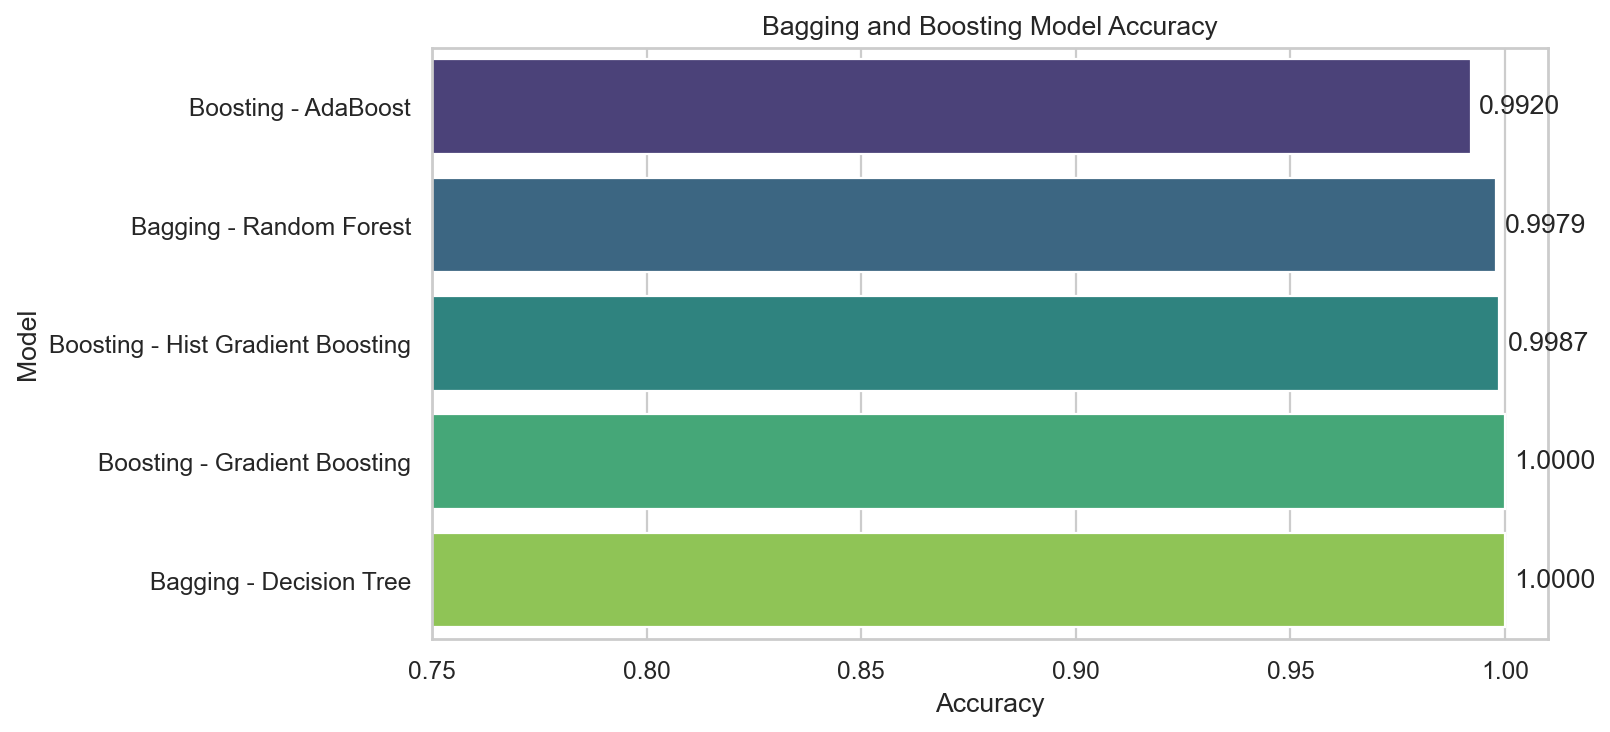
\includegraphics[width=14.0cm,height=6.4cm,keepaspectratio]{fig_04_ensemble_accuracy.png}
\caption{Bagging and Boosting model accuracy comparison.}
\label{fig:ensembleacc}
\end{figure}

\subsection{Independent Model Results}

\begin{table}[H]
\centering
\scriptsize
\caption{Independent Model Results}
\label{tab:independent}
\setlength{\tabcolsep}{3pt}
\renewcommand{\arraystretch}{1.28}
\begin{tabularx}{\linewidth}{|C{0.65cm}|Y|C{1.35cm}|C{1.35cm}|C{1.2cm}|C{1.25cm}|}
\hline
\rowcolor{SOAlightblue}
\textbf{Rank} & \textbf{Model} & \textbf{Accuracy} & \textbf{Precision} & \textbf{Recall} & \textbf{F1-Score}\\
\hline
1 & \textbf{Random Forest} & \textbf{0.9979} & \textbf{0.9962} & \textbf{1.0000} & \textbf{0.9981}\\\hline
2 & Isolation Forest & 0.7797 & 0.7168 & 1.0000 & 0.8350\\\hline
3 & One-Class SVM & 0.7771 & 0.7144 & 1.0000 & 0.8334\\\hline
4 & Autoencoder & 0.8158 & 0.9462 & 0.7100 & 0.8113\\\hline
\end{tabularx}
\normalsize
\end{table}

\begin{table}[H]
\centering
\scriptsize
\caption{Interpretation of Independent Model Results}
\label{tab:independent_interpretation}
\setlength{\tabcolsep}{4pt}
\renewcommand{\arraystretch}{1.25}
\begin{tabularx}{\linewidth}{|L{3.4cm}|Y|}
\hline
\rowcolor{SOAlightblue}
\textbf{Model} & \textbf{Interpretation}\\
\hline
Random Forest & Best overall. It matched the EDA intuition because tree splits captured port behavior, byte/packet volume, connection-state patterns, and missing-value indicators.\\\hline
Isolation Forest & Detected all malicious traffic, giving perfect recall, but produced more false positives because it treats many unusual benign records as anomalies.\\\hline
One-Class SVM & Also achieved perfect recall, but lower precision. Better results may require careful tuning of kernel, \texttt{nu}, gamma, and normal-sample selection.\\\hline
Autoencoder & High precision but lower recall. It may need better hidden-layer depth, threshold selection, regularization, more epochs, and more benign-only training data.\\\hline
\end{tabularx}
\normalsize
\end{table}

\begin{figure}[H]
\centering
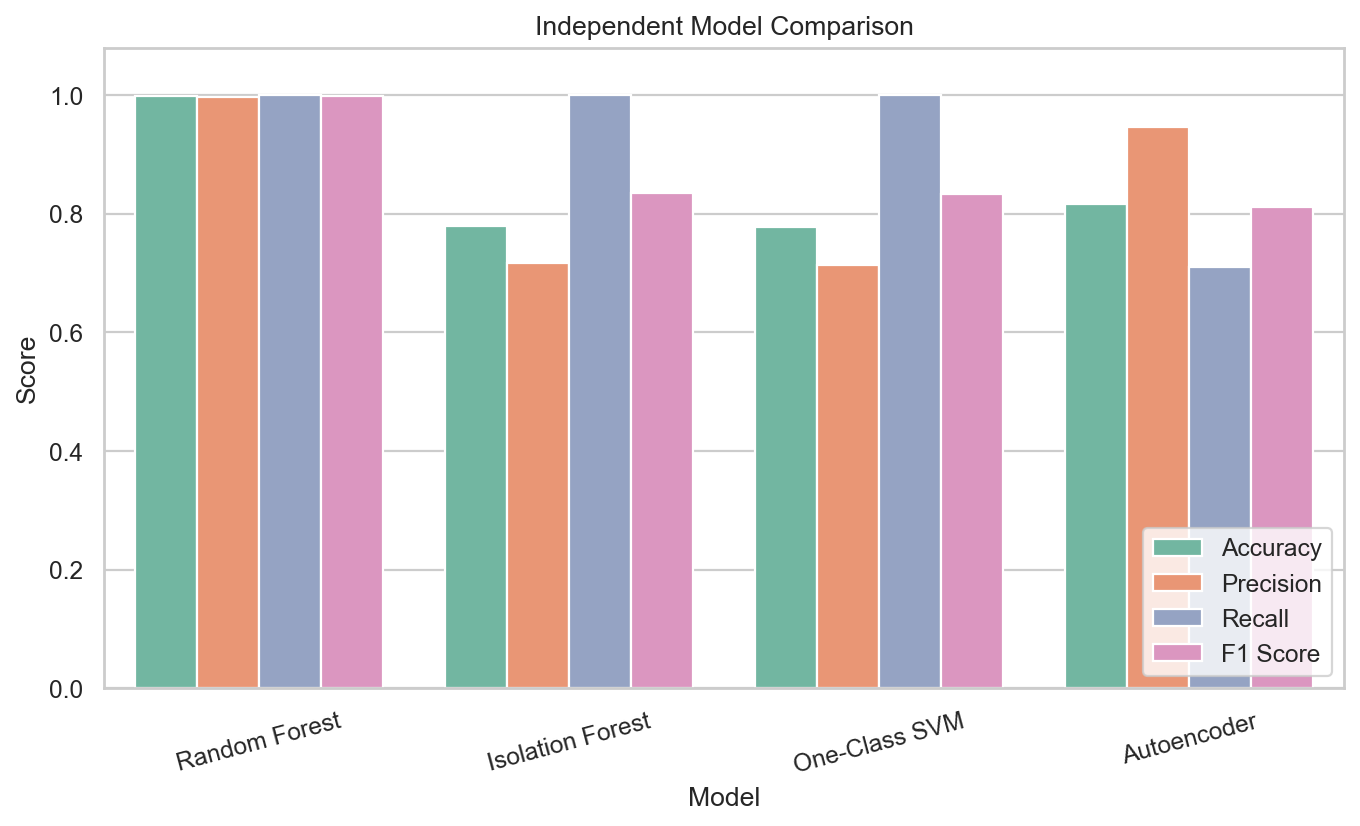
\includegraphics[width=14.0cm,height=7.8cm,keepaspectratio]{fig_05_independent_model_metrics.png}
\caption{Independent model comparison across accuracy, precision, recall, and F1-score.}
\label{fig:indmetrics}
\end{figure}

\begin{mdframed}[style=infobox]
\centering
\textbf{Best Final Model: Random Forest}\\[4pt]
\begin{tabular}{C{2.8cm}C{2.8cm}C{2.8cm}C{2.8cm}}
\textbf{Accuracy} & \textbf{Precision} & \textbf{Recall} & \textbf{F1-Score}\\
0.9979 & 0.9962 & 1.0000 & 0.9981
\end{tabular}\\[5pt]
\small Saved as: \texttt{best\_network\_anomaly\_model.pkl}
\end{mdframed}

% ============================================================
\section{Streamlit Web Application}

\subsection{Application Overview}
Streamlit was used to convert the trained machine learning model into a usable web application. The application loads the saved \texttt{.pkl} model and allows users to predict whether traffic is benign or malicious.

\subsection{Implemented App Features}
\begin{itemize}
  \item \textbf{Model loading:} Loads \texttt{best\_network\_anomaly\_model.pkl} using Joblib.
  \item \textbf{Manual prediction:} User enters one network traffic record through a form.
  \item \textbf{testing\_data.csv prediction:} User selects one row from testing data and compares actual vs predicted label.
  \item \textbf{Feature preparation:} Uses the same feature engineering logic as the notebook.
  \item \textbf{Prediction display:} Shows Benign or Malicious result.
  \item \textbf{Confidence chart:} Shows prediction probability when supported by the model.
  \item \textbf{Traffic visualizations:} Displays byte volume, packet volume, and port summary.
  \item \textbf{Sidebar:} Shows model status, project information, and label guide.
  \item \textbf{Error handling:} Displays readable messages for model-loading or version mismatch errors.
\end{itemize}

\subsection{How to Run}
\begin{lstlisting}[style=bashcode]
cd D:\MLC_Projects
python -m streamlit run app.py
\end{lstlisting}

\begin{figure}[H]
\centering
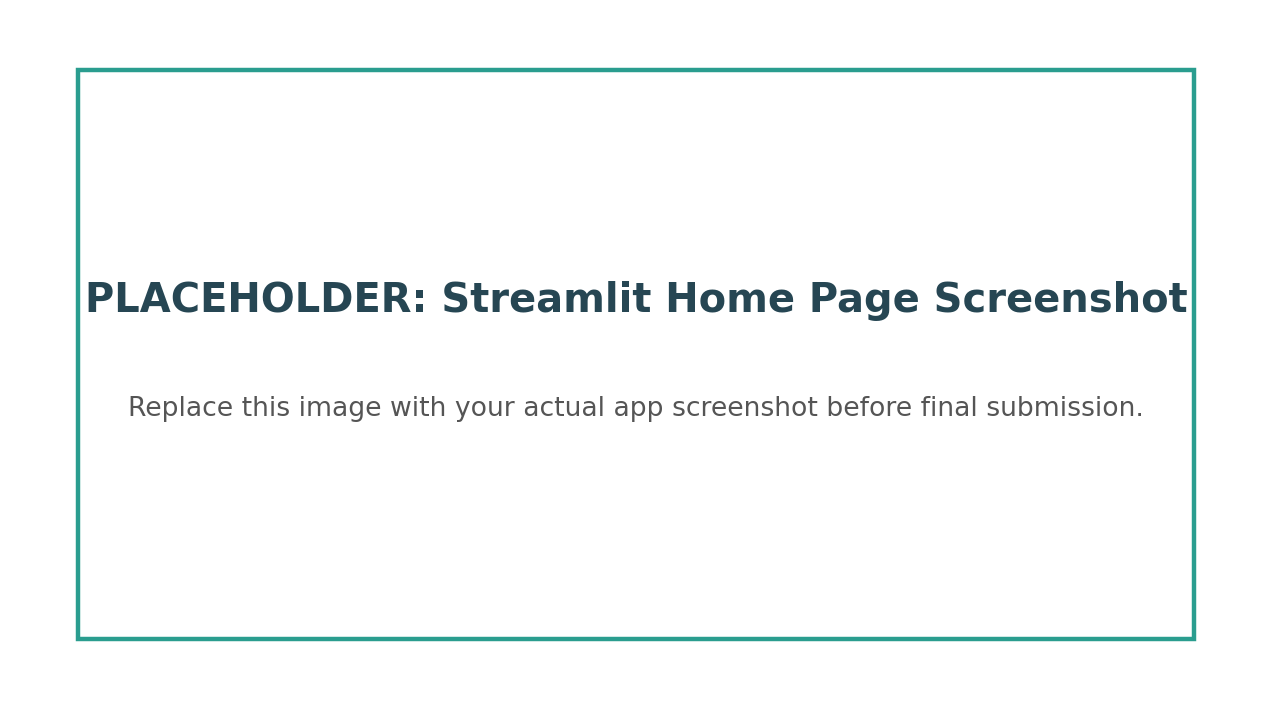
\includegraphics[width=0.9\linewidth]{placeholder_streamlit_home.png}
\caption{Placeholder for Streamlit home page screenshot. Replace with actual screenshot.}
\label{fig:sthome}
\end{figure}

\begin{figure}[H]
\centering
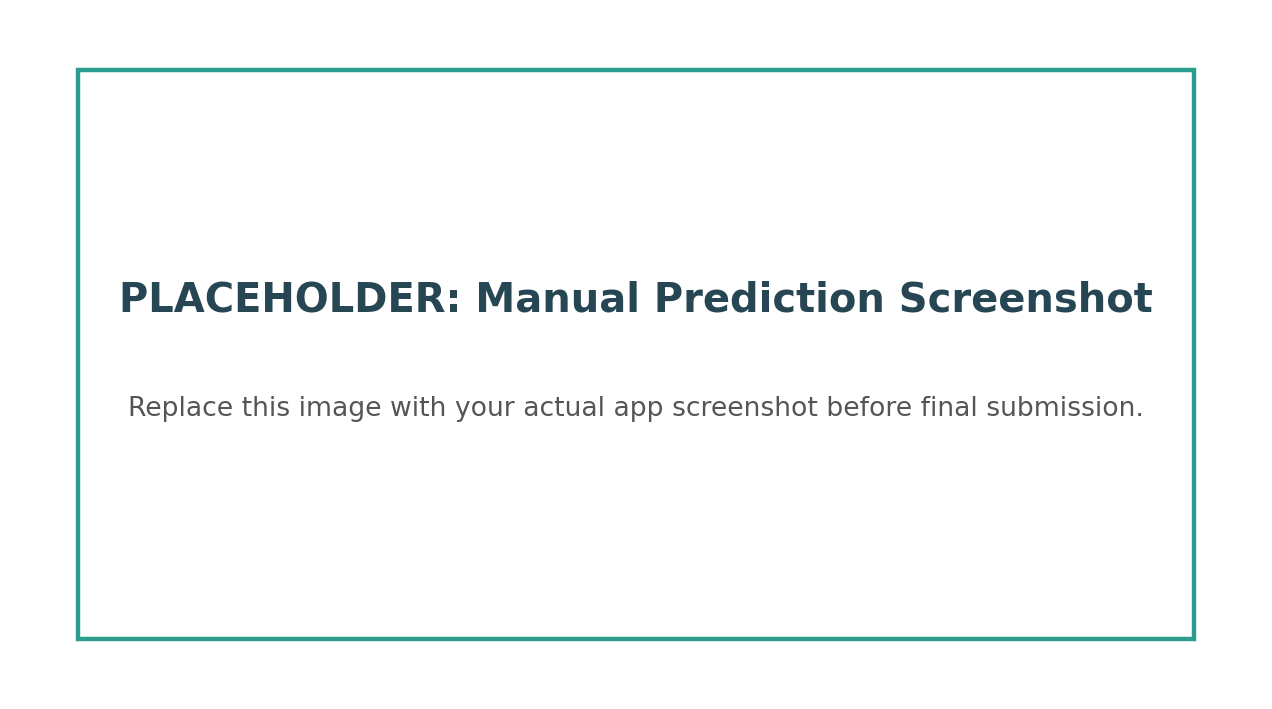
\includegraphics[width=0.9\linewidth]{placeholder_manual_prediction.png}
\caption{Placeholder for manual prediction screenshot. Replace with actual screenshot.}
\label{fig:manual}
\end{figure}

\begin{figure}[H]
\centering

\includegraphics[width=0.9\linewidth]{placeholder_csv_prediction.png}
\caption{Placeholder for testing-data row prediction screenshot. Replace with actual screenshot.}
\label{fig:csv}
\end{figure}

% ============================================================
\section{Applications}

\begin{itemize}
  \item \textbf{Enterprise Network Monitoring:} The model can act as a first-level detector for suspicious connections in organizational traffic.
  \item \textbf{IoT Device Protection:} IoT devices are common malware targets; this system can help identify botnet-like communication and scanning behavior.
  \item \textbf{Smart City Infrastructure:} Traffic from cameras, sensors, and gateways can be monitored for abnormal patterns.
  \item \textbf{Cloud Traffic Anomaly Detection:} Cloud network logs can be processed to detect lateral movement and suspicious service access.
  \item \textbf{Cybersecurity Education:} The project demonstrates the complete ML workflow from dataset to deployed app.
  \item \textbf{Preliminary IDS Dashboard:} The Streamlit app can be extended as a dashboard for analysts to inspect suspicious records.
  \item \textbf{Research Baseline:} Results can be compared with future models, larger datasets, or new feature engineering methods.
\end{itemize}

% ============================================================
\section{Limitations}

\begin{itemize}
  \item Only 50,000 records were used for this implementation, so training on the full IoT-23 dataset may change performance.
  \item The model is trained on selected IoT-23 traffic and may require retraining for other networks, devices, or malware families.
  \item Real-time packet capture is not implemented in the current app; the app works on manual input and selected CSV rows.
  \item The app currently predicts one manually entered record or one selected testing-data row at a time.
  \item Autoencoder performance depends heavily on hidden-layer design, threshold selection, training epochs, and benign-only training quality.
  \item One-Class SVM can be slow for large datasets and requires tuning of kernel, gamma, and \texttt{nu}.
  \item The saved \texttt{.pkl} file requires compatible Scikit-learn versions; otherwise model loading can fail.
  \item Very high accuracy may also indicate that the selected dataset split contains strongly separable patterns; future testing should include more scenarios and real simulated attacks.
\end{itemize}

% ============================================================
\section{Future Scope}

\begin{itemize}
  \item Add batch CSV upload prediction in Streamlit so many network records can be tested together.
  \item Integrate real-time packet capture using tools such as Zeek, Scapy, Tshark, or Wireshark exports.
  \item Simulate real-life attacks in a safe lab environment using tools such as Nmap, Hping3, Metasploit test machines, and Kali Linux. The captured traffic can then be converted into Zeek-style logs and tested against the trained model.
  \item Test the model against real-life attack categories such as port scanning, brute-force attempts, denial-of-service traffic, malware command-and-control communication, and suspicious IoT device behavior.
  \item Train on more IoT-23 scenarios and additional datasets such as CICIDS or NSL-KDD for broader generalization.
  \item Add explainable AI using SHAP or LIME to show why a record was classified as malicious.
  \item Add alerting through email, dashboard notifications, or SIEM integration.
  \item Deploy the Streamlit app on Streamlit Community Cloud or a cloud server.
  \item Optimize Autoencoder architecture using more hidden layers, dropout, regularization, and threshold tuning.
  \item Add continuous retraining when new labeled traffic becomes available.
\end{itemize}

% ============================================================
\section{Conclusion}

The \textbf{MLC Network Detection System} successfully demonstrates a complete machine learning workflow for network anomaly detection. The project uses IoT-23 traffic data, performs cleaning and EDA, creates meaningful engineered features, trains multiple models, evaluates them with proper metrics, saves the best model, and deploys it using Streamlit.

Random Forest was selected as the final model because it achieved the best independent result with Accuracy 0.9979, Precision 0.9962, Recall 1.0000, and F1-score 0.9981. This strong performance is aligned with the EDA intuition: the dataset contains rule-like patterns in ports, packet counts, byte ratios, connection state, and missing-value indicators, which tree-based ensembles capture effectively.

The final Streamlit application makes the system interactive and practical by supporting both manual prediction and prediction from \texttt{testing\_data.csv}. This project shows how machine learning can support adaptive cybersecurity and intelligent network monitoring.

% ============================================================
\section*{References}
\addcontentsline{toc}{section}{References}

\small
\begin{enumerate}[label={[\arabic*]},leftmargin=2em,itemsep=3pt]
  \item S. García, M. Parmisano, and M. J. Erquiaga, ``IoT-23: A labeled dataset with malicious and benign IoT network traffic,'' Zenodo, 2020. \url{https://doi.org/10.5281/zenodo.4743746}
  \item Stratosphere Laboratory, ``IoT-23 Dataset,'' Czech Technical University. \url{https://www.stratosphereips.org/datasets-iot23}
  \item L. Breiman, ``Random Forests,'' Machine Learning, vol. 45, no. 1, pp. 5--32, 2001. \url{https://doi.org/10.1023/A:1010933404324}
  \item F. T. Liu, K. M. Ting, and Z.-H. Zhou, ``Isolation Forest,'' IEEE ICDM, 2008. \url{https://doi.org/10.1109/ICDM.2008.17}
  \item B. Schölkopf et al., ``Estimating the Support of a High-Dimensional Distribution,'' Neural Computation, 2001. \url{https://doi.org/10.1162/089976601750264965}
  \item M. Sakurada and T. Yairi, ``Anomaly Detection Using Autoencoders with Nonlinear Dimensionality Reduction,'' MLSDA, 2014. \url{https://doi.org/10.1145/2689746.2689747}
  \item Scikit-learn Documentation. \url{https://scikit-learn.org/stable/}
  \item Streamlit Documentation. \url{https://docs.streamlit.io/}
  \item Pandas Documentation. \url{https://pandas.pydata.org/docs/}
  \item TensorFlow Documentation. \url{https://www.tensorflow.org/}
\end{enumerate}
\normalsize

% ============================================================
\newpage
\section*{Appendix: Important Code Snippets}
\addcontentsline{toc}{section}{Appendix: Important Code Snippets}

\subsection*{Data Loading}
\begin{lstlisting}[style=pycode]
df = pd.read_csv(
    file_path,
    sep="\t",
    skiprows=8,
    names=columns,
    nrows=50_000,
    na_values=["-", "", "(empty)"],
    low_memory=False,
)
\end{lstlisting}

\subsection*{Feature Engineering}
\begin{lstlisting}[style=pycode]
def engineer_features(data):
    data = data.copy()
    for col in ["service", "history", "orig_bytes", "resp_bytes"]:
        data[f"{col}_missing"] = data[col].isna().astype(int)

    ts = pd.to_datetime(data["ts"], unit="s", errors="coerce")
    data["hour"] = ts.dt.hour
    data["dayofweek"] = ts.dt.dayofweek

    data["total_bytes"] = data["orig_bytes"].fillna(0) + data["resp_bytes"].fillna(0)
    data["total_pkts"] = data["orig_pkts"].fillna(0) + data["resp_pkts"].fillna(0)
    data["bytes_per_pkt"] = data["total_bytes"] / data["total_pkts"].replace(0, np.nan)
    data["orig_resp_byte_ratio"] = data["orig_bytes"] / data["resp_bytes"].replace(0, np.nan)
    data["orig_resp_pkt_ratio"] = data["orig_pkts"] / data["resp_pkts"].replace(0, np.nan)
    data["orig_port_is_well_known"] = (data["id.orig_p"] <= 1024).astype(int)
    data["resp_port_is_well_known"] = (data["id.resp_p"] <= 1024).astype(int)
    data["orig_ip_prefix"] = data["id.orig_h"].astype(str).str.extract(r"^(\d+\.\d+)", expand=False)
    data["resp_ip_prefix"] = data["id.resp_h"].astype(str).str.extract(r"^(\d+\.\d+)", expand=False)
    return data.drop(columns=["uid", "label", "id.orig_h", "id.resp_h", "ts"], errors="ignore")
\end{lstlisting}

\subsection*{Model Saving}
\begin{lstlisting}[style=pycode]
import joblib
joblib.dump(best_model, "best_network_anomaly_model.pkl")
\end{lstlisting}

\subsection*{Streamlit Run Command}
\begin{lstlisting}[style=bashcode]
python -m streamlit run app.py
\end{lstlisting}

\end{document}
